%
% $Id: $
%
%
% Compilar a .pdf con LaTeX (pdflatex)
% Es necesario instalar Beamer (paquete latex-beamer en Debian)
%

%
% Gr�ficos:
% Los gr�ficos pueden suministrarse en PNG, JPG, TIF, PDF, MPS
% Los EPS deben convertirse a PDF (usar epstopdf)
%

\documentclass{beamer}
\usetheme{GSyC}
\usepackage[latin1]{inputenc}
\usepackage{graphics}
\usepackage{amssymb} % Simbolos matematicos


%% Metadatos del PDF.
\hypersetup{
  pdftitle={Protocolos para la Transmisi�n de Audio y V�deo por Internet},
  pdfauthor={Gregorio Robles, Jes�s M. Gonz�lez Barahona},
  pdfcreator={GSyC, Universidad Rey Juan Carlos},
  pdfproducer=PDFLaTeX,
  pdfsubject={Protocolos para la Transmisi�n de Audio y V�deo por Internet},
}
%%

\begin{document}

\title{El Jitter en Tiempo Real}
\subtitle{Protocolos para la Transmisi�n de Audio y V�deo en Internet}
\institute{grex@gsyc.urjc.es \\
GSyC, Universidad Rey Juan Carlos}
\author{Gregorio Robles}
\date[Nov 2014]{12 de noviembre de 2014}

\frame{
\maketitle
}


% Si el titulo o el autor se quieren acortar para los pies de p�gina
% se pueden redefinir aqu�:
%\title{Titulo corto}
%\author{Autores abreviado}


%% LICENCIA DE REDISTRIBUCION DE LAS TRANSPAS
\frame{
~
\vspace{4cm}

\begin{flushright}
{\tiny
(cc) 2013-4 Gregorio Robles, Jes�s M. Gonz�lez Barahona \\
  Some rights reserved. This work licensed under Creative Commons \\
  Attribution-ShareAlike License. To view a copy of full license, see \\
\ \\
  http://creativecommons.org/licenses/by-sa/3.0/ or write to \\
  Creative Commons, 559 Nathan Abbott Way, Stanford, \\
  California 94305, USA. \\
\ 
}
\end{flushright}
}
%%

%--------------------------------------------------------

\begin{frame}
\frametitle{�Qu� es el \emph{jitter}?}

\begin{itemize}
  \item Es la variabilidad del tiempo entre paquetes
  \item Es un efecto de enviar informaci�n en redes de ordenadores
  \begin{itemize}
    \item Aunque tambi�n puede haber jitter en la fuente
  \end{itemize}
  \item Puede resultar molesto para usuarios de servicios en tiempo real (suenan \emph{chasquidos} al hablar).
\end{itemize}

\end{frame}



%--------------------------------------------------------
\begin{frame}
\frametitle{El jitter visualmente}

\begin{figure}[t!]
\begin{center}
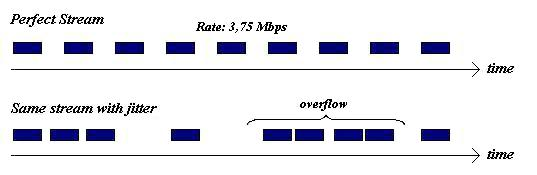
\includegraphics[width=11cm]{figs/Time_jitter.JPG}
% http://upload.wikimedia.org/wikipedia/commons/1/10/Time_jitter.JPG
\end{center}
\caption{El jitter visualmente}
\label{fig:jitter}
\end{figure}

\end{frame}


%--------------------------------------------------------
\begin{frame}
\frametitle{Recepci�n con jitter}

\begin{figure}[t!]
\begin{center}
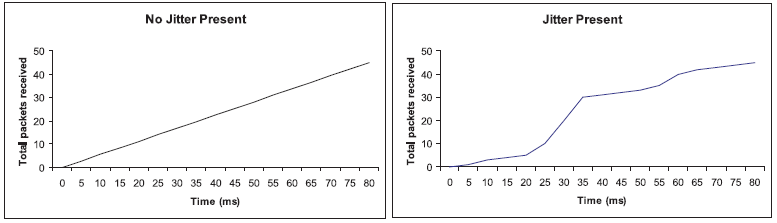
\includegraphics[width=11cm]{figs/Jitter_effects_hor.PNG}
% http://upload.wikimedia.org/wikipedia/en/b/b4/Jitter_effects_hor.PNG
\end{center}
\caption{Debido al jitter, no recibimos peri�dicamente}
\label{fig:jitter}
\end{figure}

\end{frame}


%--------------------------------------------------------

\begin{frame}
\frametitle{�C�mo se calcula el jitter?}

La f�rmula de jitter (del RFC 3550, de RTP) es:

\begin{center}
$J_i = J_{i-1} + \frac{|D_{(i-1,i)}| - J_{i-1}}{16}$
\end{center}

siendo:

\begin{center}
$D_{(i,j)} = (R_j - S_j) - (R_i - S_i) = (R_j - R_i) - (S_j - S_i)$
\end{center}

donde:

$R_j$: tiempo de recepci�n de paquete j

$R_i$: tiempo de recepci�n de paquete i

$S_j$: tiempo de env�o de paquete j

$S_i$: tiempo de env�o de paquete j

$J_i$: Jitter del paquete i

\end{frame}


%--------------------------------------------------------
\begin{frame}
\frametitle{Un ejemplo}

\begin{figure}[t!]
\begin{center}
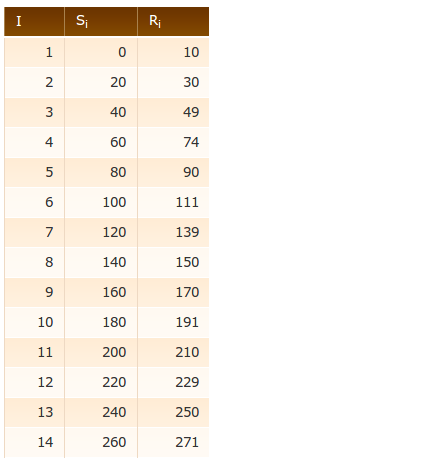
\includegraphics[width=6cm]{figs/calculo3.png}
% http://toncar.cz/Tutorials/VoIP/VoIP_Basics_Jitter.html
\end{center}
\caption{Calculando el jitter}
\label{fig:jitter3}
\end{figure}

\end{frame}


%--------------------------------------------------------
\begin{frame}
\frametitle{Un ejemplo (medio) solucionado}

\begin{figure}[t!]
\begin{center}
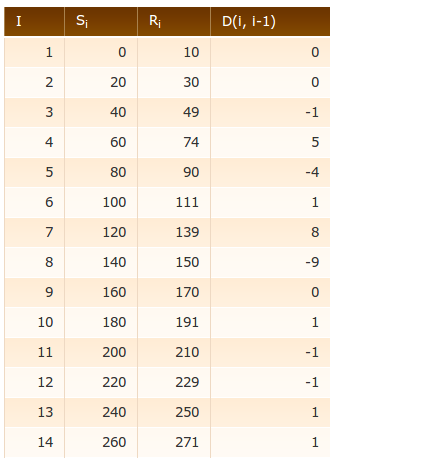
\includegraphics[width=6cm]{figs/calculo.png}
% http://toncar.cz/Tutorials/VoIP/VoIP_Basics_Jitter.html
\end{center}
\caption{Calculando el jitter}
\label{fig:jitter1}
\end{figure}

\end{frame}


%--------------------------------------------------------
\begin{frame}
\frametitle{Un ejemplo solucionado}

\begin{figure}[t!]
\begin{center}
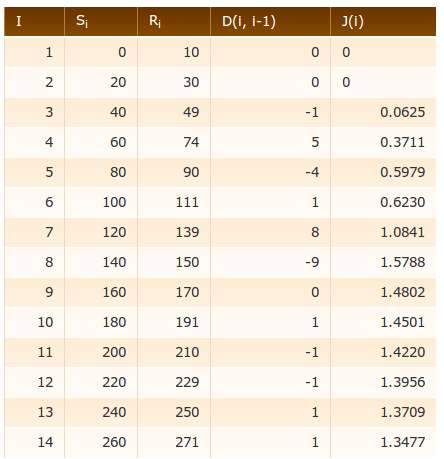
\includegraphics[width=6cm]{figs/calculo2.png}
% http://toncar.cz/Tutorials/VoIP/VoIP_Basics_Jitter.html
\end{center}
\caption{Calculando el jitter}
\label{fig:jitter2}
\end{figure}

\end{frame}

%--------------------------------------------------------

\begin{frame}
\frametitle{�Qu� es el \emph{jitter buffer}?}

\begin{itemize}
  \item Es un tiempo de espera antes de reproducir el contenido de
        los paquetes
  \item Ha de ser $< 100 ms$ en tiempo real para asegurar la calidad
  \item Para no perder ning�n paquete, su valor deber�a ser el del paquete
con mayor retraso
  \item En condiciones de red gaussiana:
    \begin{itemize}
      \item Si el valor de jitter buffer es el
de jitter perdemos un 35\% de los paquetes.
      \item Con un jitter buffer de 2 * jitter,
la p�rdida es el 6\%.
      \item Con un jitter buffer de 3 * jitter, del 2\%.
    \end{itemize}
  \item Por eso, muchas veces tendremos que aceptar alguna p�rdida.
\end{itemize}

\end{frame}



%--------------------------------------------------------

\frame{
\maketitle
}

\end{document}
